After implementing our system, the next step is conducting experiments. This will assist in evaluating and validating our thesis results.
We focus on quantitative and qualitative results. To present our quantitative results we will use Average Precision (AP) at mean Intersection over Union (mIoU) thresholds of 
25\% (AP\textsubscript{25}), 50\% (AP\textsubscript{50}), and AP,  the average over
different IoU thresholds from 0.5 to 0.95 with a step of 0.05 and for qualitative results will present a few of the point cloud segmentation and scene graphs generated using our system. We present the results in 
three parts. The first part illustrates the qualitative results of the scene graph generation method used, we show two scene graphs generated from two different datasets.
The second part illustrates the quantitative as well as qualitative results of Mask3D trained on our merged dataset, we present AP, AP\textsubscript{50} and AP\textsubscript{25} values and some 
snapshots of the final part-segmentation for a few objects. The final part showcases the qualitative results for integrating Mask3D with ConceptGraphs in order to
tackle the task two from SceneFun3D, task-driven affordance grounding.

\textit{Dataset used:}For experiments, we have used the ARKITscenes dataset. They provide a large number of scenes enumerated by visit ID and each visit ID has at most three 
video recordings of the same scene denoted by video ID. For the purpose of experiments we divide the dataset into train, validation and test splits. We have trained
the Mask3D and PointNet++ models with a training set and validation set. Therefore, for experimentation, we will use the test split and evaluate the two SceneFun3D tasks defined 
earlier. 
\begin{figure}[ht!]
    \centering
    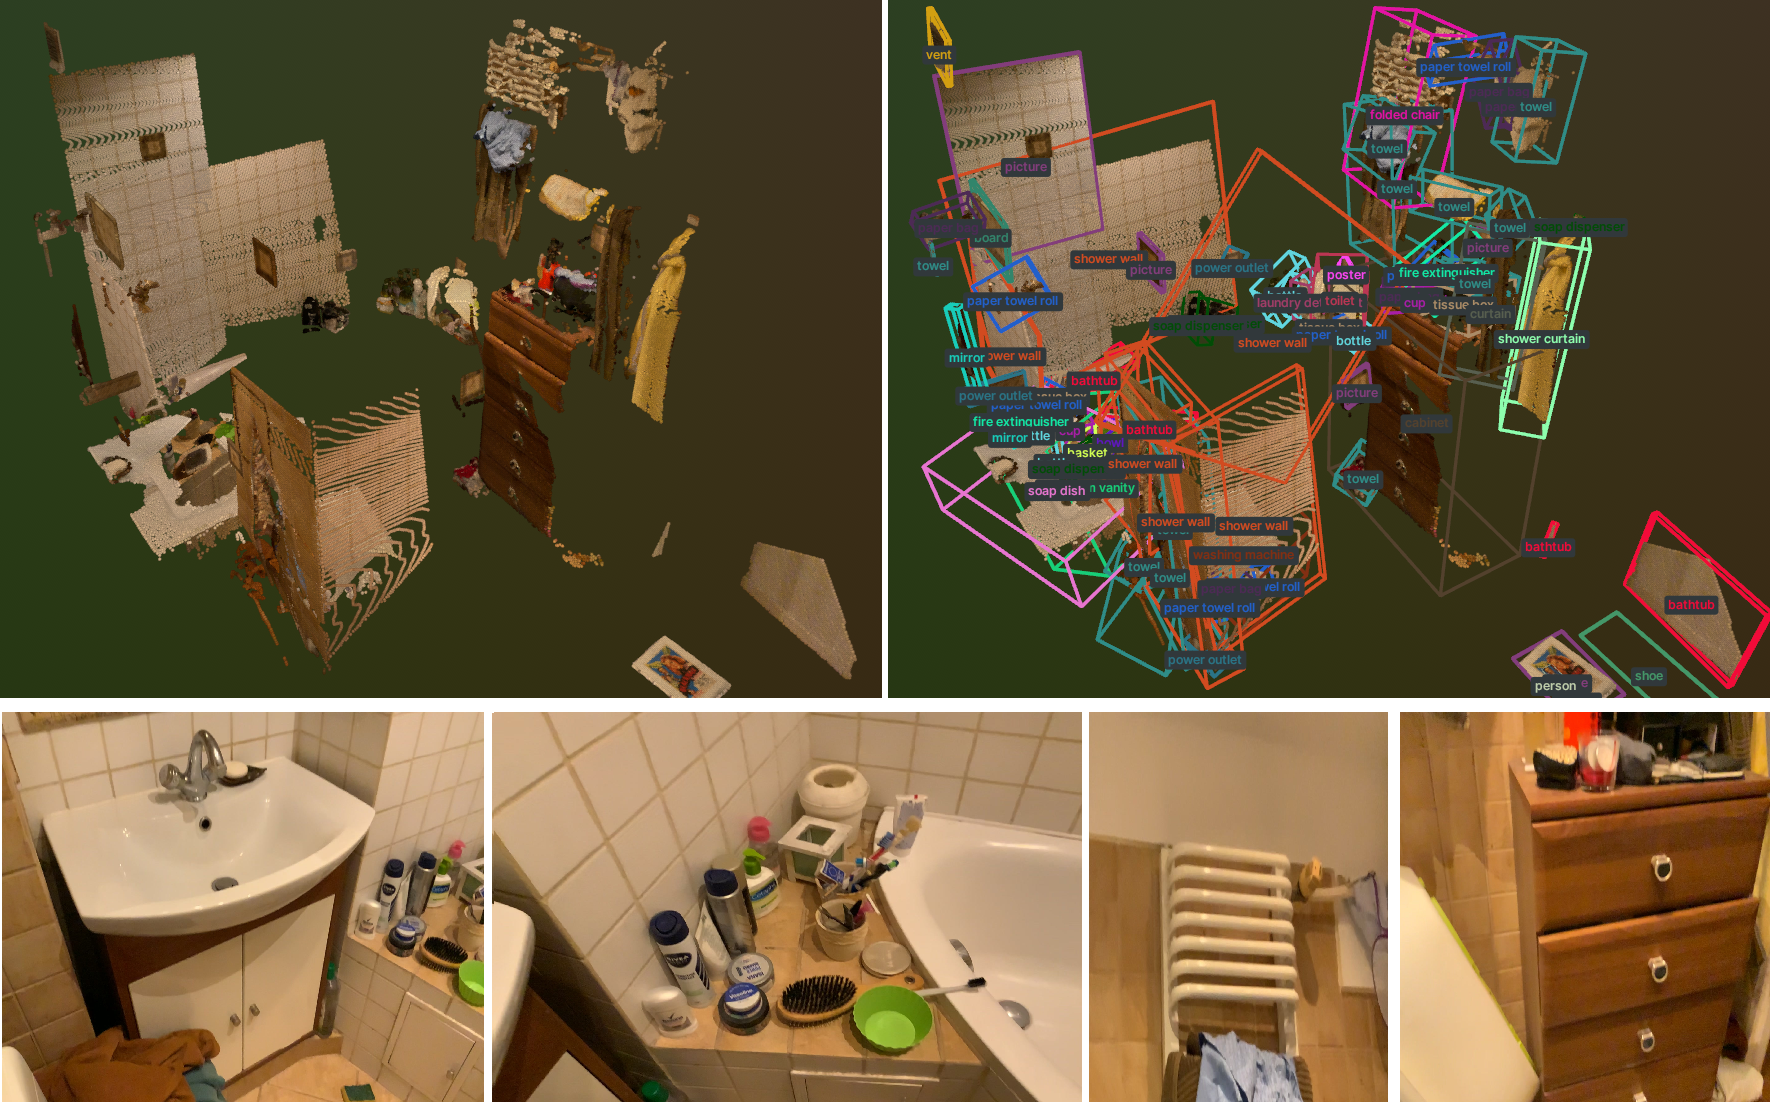
\includegraphics[width=\textwidth]{content/images/results/SF_SG.png}
    \caption{Scene graph of a scene from ARKITscenes (visit\_id 468074, video\_id 47333827)}
    \label{fig:result1}
\end{figure}
\section{Scene graph generation on real-world dataset}
\label{sec:SG}
One of the milestones of this thesis was to generate a scene graph using the dataset captured live, i.e. a real-world dataset. We performed experiments related to
 this task using two approaches. The first approach was to utilise the already recorded SceneFun3D dataset which has real-world scenes. The second approach was 
to capture our dataset using the Intel Realsense camera in our own Socially Intelligent Robotics (SIR) lab at the Institute of Artificial Intelligence, 
University of Stuttgart. We present the qualitative results for both of these approaches by showing some snaps of the final scene graphs generated 
using our system. \cref{fig:result1} is the scene graph for the SceneFun3D dataset for video\_id\: 47333827 and visit\_id\: 468074. \cref{fig:result2} 
depicts the scene graph from one of the office in our SIR lab. This scene was captured using Intel Realsene D435 Depth camera. The recording was done manually.
The final scene graphs does not include background classes such as  floor, wall and ceilings.

\begin{figure}[ht!]
    \centering
    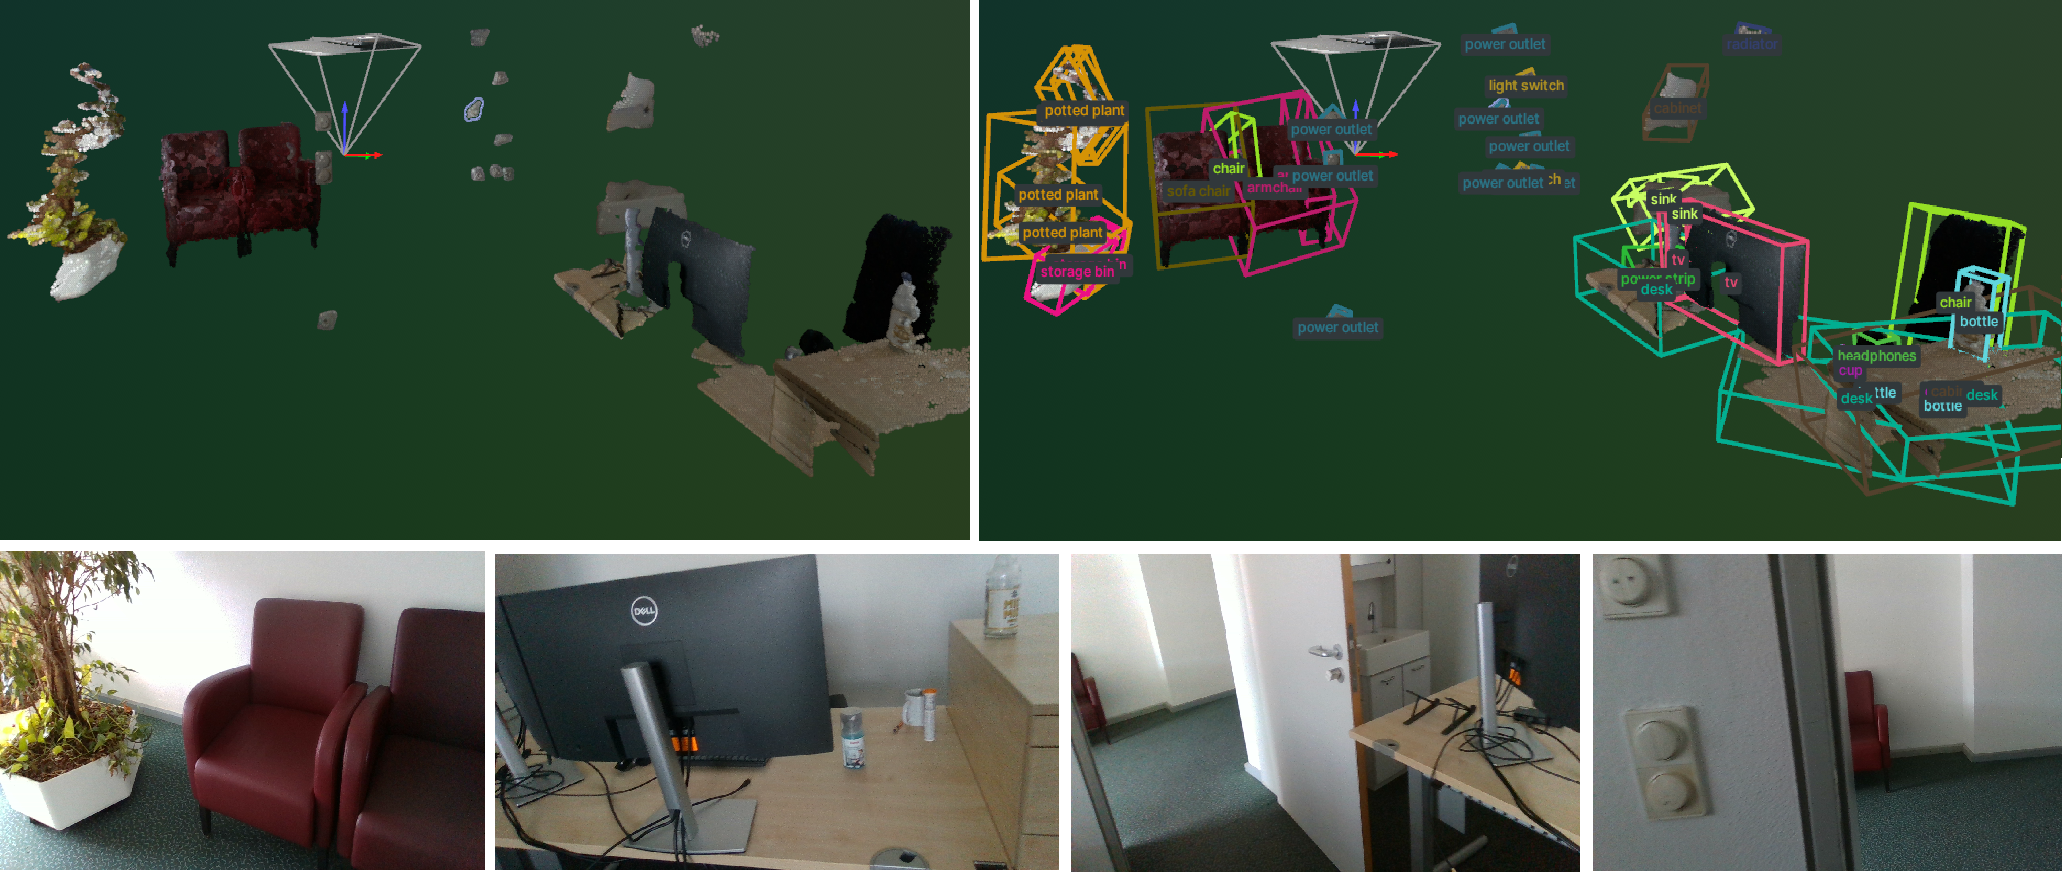
\includegraphics[width=\textwidth]{content/images/results/SIR_SG.png}
    \caption{Scene graph of SIR lab.}
    \label{fig:result2}
\end{figure}
\section{Functionality segmentation}
\label{sec:FS}
For this task, we will present both the quantitative results as well as the qualitative results. The results from SceneFun3D for this task are taken as a baseline. 
SceneFun3D have adapted Mask3D for this task. They also compare SoftGroup and LERF. We have utilised Mask3D and PointNet++ in our experiments. The reason for using 
Mask3D was to compare the results with SceneFun3D and evaluate our method. PointNet ++ was also leveraged for this task but we present qualitative results for PointNet++.

The \cref{tab:quantitativeResults} compares the results from SceneFun3D and our experiments. We also consider all the results from SceneFun3D and do not only limit ourselves to
Mask3D. 

\begin{longtable}{l|l|l|l}
    \caption{Quantitative result comparison for task functionality segmentation.} \label{tab:quantitativeResults} \\
    \hline \multicolumn{1}{|c|}{\textbf{Method}} & \multicolumn{1}{c|}{\textbf{AP}} & \multicolumn{1}{c|}{\textbf{AP\textsubscript{50}}} & \multicolumn{1}{c|}{\textbf{AP\textsubscript{25}}} \\ \hline
    SoftGroup-F & 3.6 & 17.2 & 11 \\
    LERF & 4.8 & 12.3 & 18.1\\
    Mask3D-F & 7.9 & 18.3 & 26.6\\
    Mask3D-Ours & \textbf{20.5} & \textbf{28.3} & \textbf{32.2}\\
    \hline
\end{longtable}
\begin{longtable}{l|l|l|l}
    \caption{Quantitative results of individual affordance classes for functionality segmentation using Mask3D on merged dataset.} \label{tab:quantitativeResultsIndividual} \\
    \hline \multicolumn{1}{|c|}{\textbf{Affordance Class}} & \multicolumn{1}{c|}{\textbf{AP}} & \multicolumn{1}{c|}{\textbf{AP\textsubscript{50}}} & \multicolumn{1}{c|}{\textbf{AP\textsubscript{25}}} \\ \hline
    hook\_turn & \textbf{43.3} & \textbf{62.4} & \textbf{62.4} \\
    hook\_pull & 6.9 & 13.8 & \textbf{20.6}\\
    key\_press & 6.8 & 11.5 & \textbf{21}\\
    rotate & \textbf{24.5} & \textbf{31.7} & \textbf{34.6}\\
    foot\_push & 3.2 & \textbf{19.9} & \textbf{23.2}\\
    unplug & 3 & 3.7 & 5\\
    plug\_in & 0 & 0.1 & 0.9\\
    pinch\_pull & \textbf{15.6} & \textbf{31.2} & \textbf{41}\\
    tip\_push & 0 & 0 & 0\\
    \hline
\end{longtable}
\begin{figure}[ht!]
    \centering
    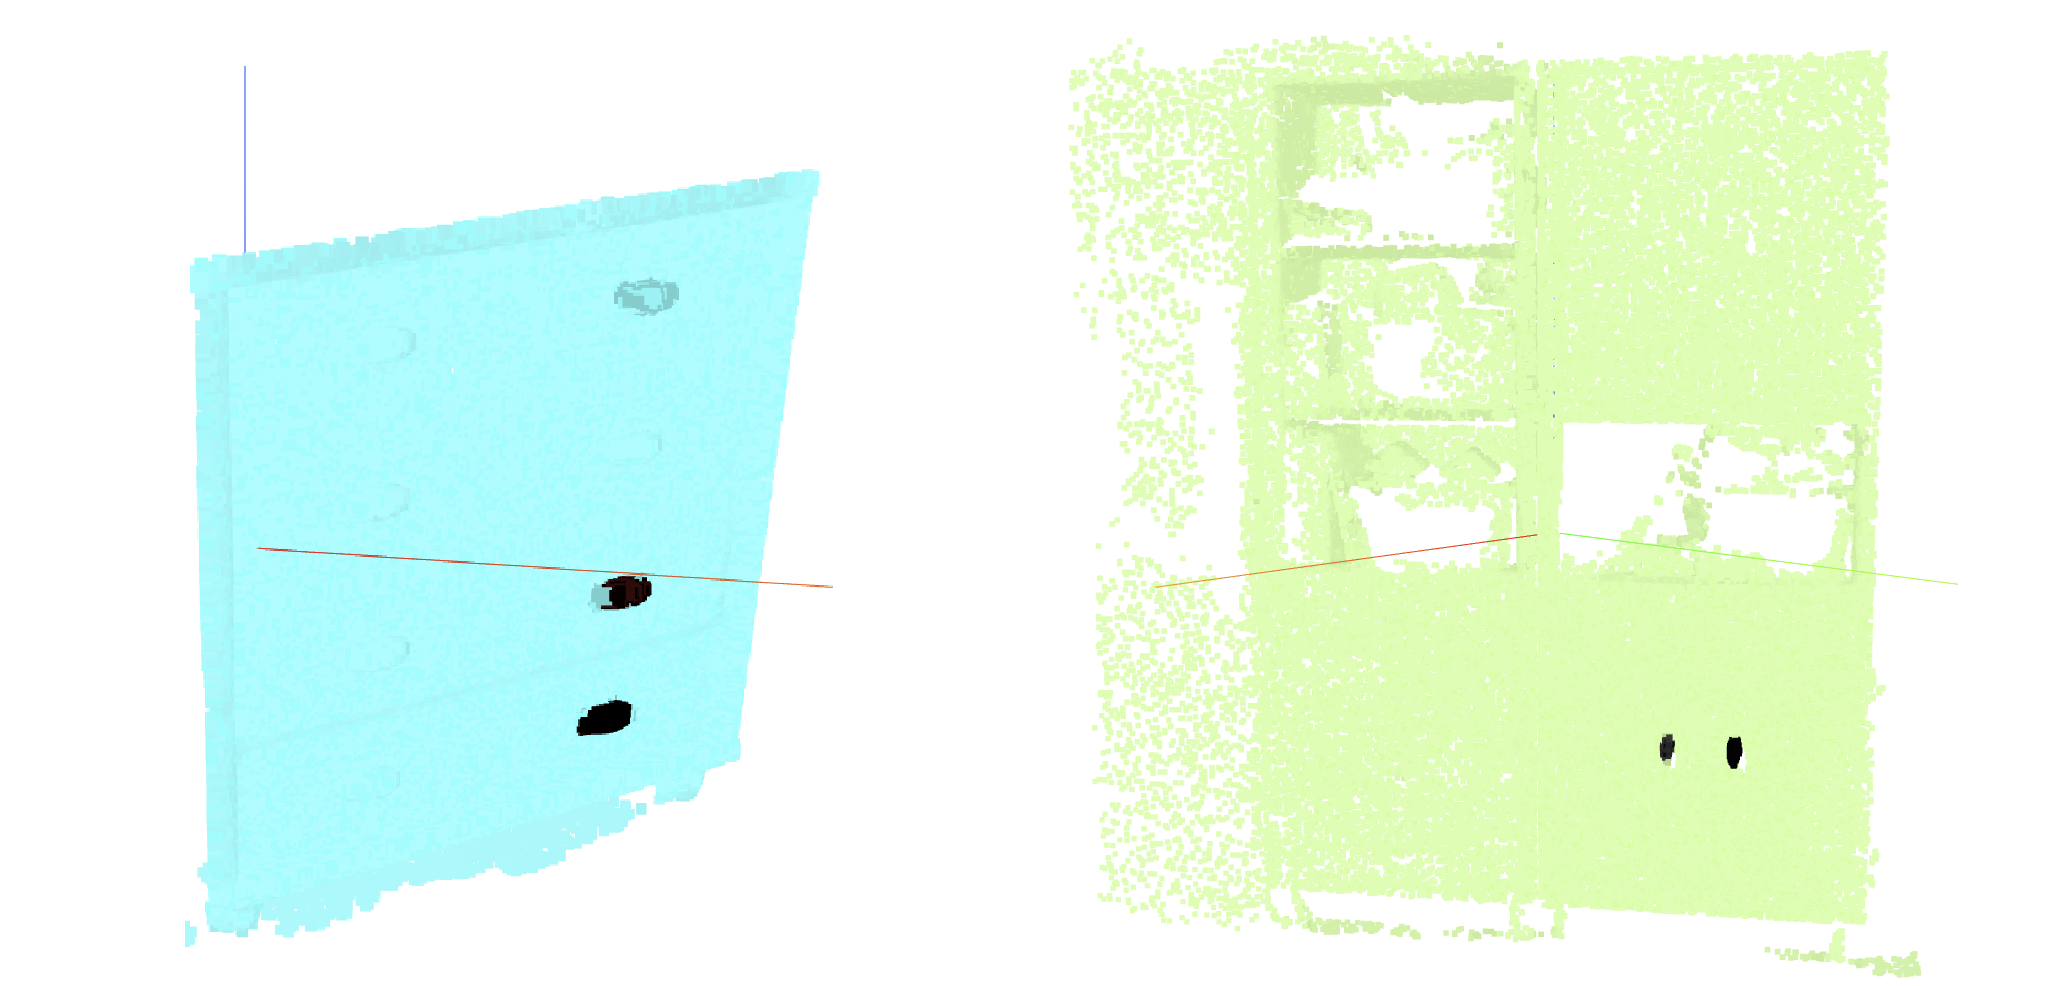
\includegraphics[width=\textwidth]{content/images/results/PartObj.png}
    \caption{Part-Object segmentation results for class pinch\_pull on ARKITscenes dataset.}
    \label{fig:task1result1}
\end{figure}

\begin{figure}[ht!]
    \centering
    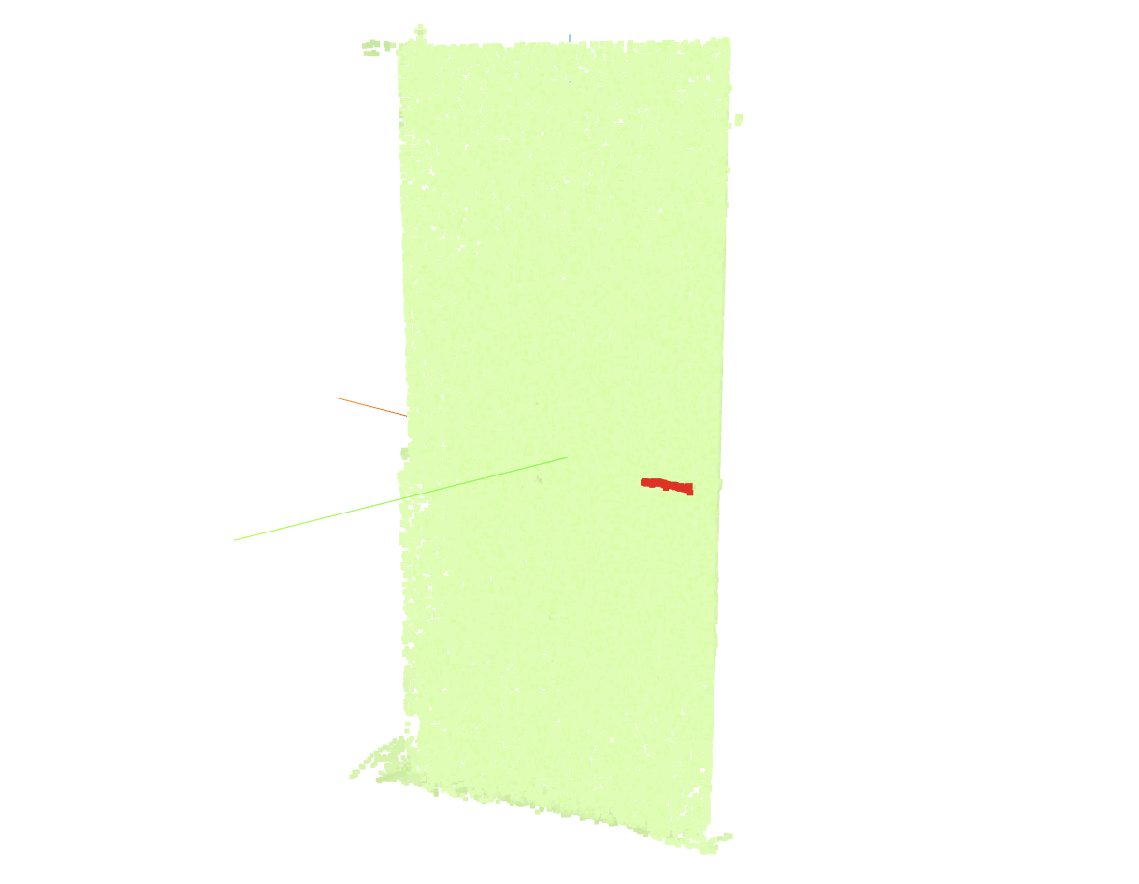
\includegraphics[width=\textwidth]{content/images/results/PartObj2.png}
    \caption{Part-Object segmentation results for class hook\_turn on ARKITscenes dataset.}
    \label{fig:task1result2}
\end{figure}
We also present the individual AP results for each affordance class in \cref{tab:quantitativeResultsIndividual}
In addition to quantitative results, let us take a look at some qualitative results in \cref{fig:task1result1} and \cref{fig:task1result2}. 
Further, \cref{fig:task1result1} shows the part-object segmentation for the affordance class \enquote{pinch\_pull}, here the parts are in black colour and
they can be afforded to be pinch pulled. \cref{fig:task1result2} shows the part-object segmentation for class \enquote{hook\_turn}, here
the part is colored red and the non functional segment is in light green.

\section{Task-driven affordance grounding}
\label{sec:TDAG}
The results for this task will be presented as qualitative results with images from the output of our system. We query our concept graph with natural language
 and expect the system to return, the segmented point cloud as a heat map with the most probable object or part in a black and 
 the least probable object or part in light blue. 

We ask our system two queries, \enquote{Open the cabinet below the washbasin} and \enquote{Open the drawer in the cabinet below heater}. 
The results for the two queries are given below in \cref{fig:taskdrivenA1} and \cref{fig:taskdrivenA2}. The \cref{fig:taskdrivenQ1} and \cref{fig:taskdrivenQ2} 
give the scenegraphs before querying for query 1 and query 2 respectively.

\begin{figure}[ht!]
    \centering
    \includegraphics[width=\textwidth]{content/images/results/taskdrivenQ1.png}
    \caption{Scene graph befor the query \enquote{Open the cabinet below the washbasin}.}
    \label{fig:taskdrivenQ1}
\end{figure}

\begin{figure}[ht!]
    \centering
    \includegraphics[width=\textwidth]{content/images/results/taskdrivenA1.png}
    \caption{Qualitative result for Task-driven affordance grounding and query \enquote{Open the cabinet below the washbasin}.}
    \label{fig:taskdrivenA1}
\end{figure}

\begin{figure}[ht!]
    \centering
    \includegraphics[width=\textwidth]{content/images/results/taskdrivenQ2.png}
    \caption{Scene graph befor the query \enquote{Open the drawer in the cabinet below heater}.}
    \label{fig:taskdrivenQ2}
\end{figure}
\begin{figure}[ht!]
    \centering
    \includegraphics[width=\textwidth]{content/images/results/taskdrivenA2.png}
    \caption{Qualitative result for Task-driven affordance grounding and query \enquote{Open the drawer in the cabinet below heater}.}
    \label{fig:taskdrivenA2}
\end{figure}

It is visible that in both of the queries the system returned the most probable part in black. For the first query, it returned the cabinet 
handle below the mirror. In the second query, it returned the drawer knobs in the cabinet which is located below the heater.


The results show, our method of generating a scene graph includes the fine-grained relationships between an object and its parts.
From \cref{sec:SG} we can see the scene graph generated for two real world datasets, the first being SceneFun3D and the second one recorded
manually at SIR lab, University of Stuttgart. The results from \cref{sec:FS} show the improvemnet in part-object segmentation as compared 
to the baseline of SceneFun3D, this was possible because the segmentation was carried out on individual objects and not on entire scene as done by
SceneFun3D. Finally, the results from \cref{sec:TDAG} depict the novel addition of part-object segmentation in scene graph.